%% ADScAI 2026 authors: use the sigconf format; do not change margins/fonts

\documentclass[sigconf,anonymous]{acmart}

% --- Rights management ---
\setcopyright{none}
\settopmatter{printacmref=false}

\AtBeginDocument{%
  \providecommand\BibTeX{{%
    Bib\TeX}}}

\acmConference[ADScAI Conference]{Second Annual Conference of Department of Computer Science & Engineering}{2026}{University of Moratuwa, Sri Lanka}
\acmYear{2026}
\acmDOI{}
\acmISBN{}

% Packages (keep only what is compatible and needed)
\usepackage[utf8]{inputenc}
\usepackage[T1]{fontenc}
\usepackage{graphicx}
\usepackage{amsmath}
\usepackage{booktabs}
\usepackage{hyperref}
\usepackage{xcolor}
\usepackage{listings}
\usepackage{tikz}
\usetikzlibrary{shapes.geometric, arrows.meta, positioning, fit, calc}
\usepackage{pgfplots}
\pgfplotsset{compat=1.18}
\usepackage{multirow}
\usepackage{enumitem}
\usepackage{balance}

\hypersetup{
    colorlinks=true,
    linkcolor=blue,
    citecolor=blue,
    urlcolor=blue
}

\lstset{
    basicstyle=\ttfamily\footnotesize,
    breaklines=true,
    frame=single,
    backgroundcolor=\color{gray!10},
    keywordstyle=\color{blue},
    commentstyle=\color{green!50!black},
    stringstyle=\color{red!70!black}
}

\title{From Intent to Scan: A Multi-Agent System for Structured Web Security Reconnaissance}

% Replace these with real authors for camera-ready.
% For review, use: \documentclass[sigconf,anonymous,review]{acmart}
\author{Himath Samarakoon}
\affiliation{
  \institution{Department of Computer Science}
  \institution{University of Moratuwa}
  \country{Sri Lanka}
}
\email{himath.22@cse.mrt.ac.lk}

\author{Saai Syvendra}
\affiliation{
  \institution{Department of Computer Science}
  \institution{University of Moratuwa}
  \country{Sri Lanka}
}
\email{saai.22@cse.mrt.ac.lk}

\begin{document}

\begin{abstract}
This paper presents a multi-agent cybersecurity system that translates natural-language requests into coordinated security scans across service discovery, web vulnerability assessment, and exploit reconnaissance. It describes the system's evolution from a monolithic single-agent architecture (V1) to a hierarchical multi-agent orchestration framework (V2). V2 comprises three specialised sub-agents, Service Discovery (Masscan and Nmap), Web Scanning (Nikto and WPScan), and Exploitation (Metasploit), coordinated by an orchestrator that maintains a dynamic task plan. A comparative evaluation against a deliberately vulnerable WordPress target indicates that separating concerns reduces redundant tool invocations, mitigates context exhaustion, and enables parallel tool execution.
\end{abstract}

\keywords{multi-agent systems, web vulnerability, cybersecurity automation, LLM-based orchestration, vulnerability scanning}

\maketitle

% ============================================================
\section{Introduction}
\label{sec:introduction}
% ============================================================

Security researchers chain the use of multiple tools within their
workflows to analyse the security posture of software.
These workflows tend to follow an iterative pattern
of executing tools, analysing results, and using that analysis
to execute targeted tools.
This cycle is continued until the target amount of information is gathered.

Today, much of this process is performed manually.
A common starting point is service discovery and fingerprinting with tools such as Nmap \cite{nmap} to identify exposed ports and protocols.
The researchers then investigate the discovered entry points, inspect responses, and refine subsequent steps based on returned headers, payload structure, error messages, and other indicators.
This approach has proven to be effective, yet time consuming, particularly when assessments involve many hosts, endpoints, or configuration variants.

In this paper, an iterative design study of an LLM-based multi-agent system for automated deployment misconfiguration detection is presented. The contributions are:

\begin{enumerate}[leftmargin=*]
    \item A characterisation of the failure modes of monolithic single-agent security scanning (V1), including tool-call hallucination and context exhaustion.
    \item A hierarchical multi-agent architecture (V2), with three specialised sub-agents coordinated by an orchestrator that maintains a dynamic task decomposition.
    \item Configurable human-in-the-loop tool-call interrupts and parallel tool execution within sub-agents, with observations on their impact on user confidence and adoption.
    \item Design-level observations on prompt optimisation, structured output for inter-agent context passing, and safety guardrails for active exploitation.
\end{enumerate}

% ============================================================
\section{Related Work}
\label{sec:related_work}
% ============================================================

\subsection{Automated Security Scanning}

Traditional security automation relies on scripted pipelines (e.g., combining Nmap, Nikto, and Metasploit in shell scripts) or commercial platforms such as Tenable Nessus, Rapid7 InsightVM, and Burp Suite. Recent work has explored LLM-driven penetration testing, including PentestGPT~\cite{deng2023pentestgpt}, which uses an LLM to guide human operators, and ReaperAI~\cite{fang2024llmagents}, which demonstrates autonomous web hacking behaviours with frontier models.

More recent systems push toward higher autonomy and multi-stage execution. AutoAttacker~\cite{xu2024autoattacker} studies LLM-guided ``hands-on-keyboard'' attack automation in post-breach settings, integrating offensive tooling within iterative agent loops. PentestAgent~\cite{shen2024pentestagent} uses multi-agent collaboration and retrieval-augmented techniques across reconnaissance, analysis, and exploitation phases. VulnBot~\cite{kong2025vulnbot} similarly decomposes penetration testing into specialised phases guided by an explicit task graph. Other autonomous workflows such as AutoPentest~\cite{henke2025autopentest} and AutoPentester~\cite{ginige2025autopentester} evaluate agent-driven pentesting on controlled scenarios (e.g., CTF-style and vulnerable VMs) and emphasise iterative planning grounded in tool output.

The work differs from prior approaches by focusing on the architectural comparison between single-agent and hierarchical multi-agent designs for security tool orchestration, and on mechanisms that improve reliability under verbose and heterogeneous tool outputs, including structured summarisation, constrained tool access per agent, and configurable human-in-the-loop interrupts.

\subsection{Multi-Agent Systems}

Hierarchical and collaborative multi-agent architectures have been applied to software engineering~\cite{hong2023metagpt}, scientific discovery~\cite{boiko2023emergent}, and general task solving~\cite{wu2023autogen}. A recurring insight is that decomposing complex tasks across specialised agents can reduce per-agent context load and improve robustness of planning and tool use. Recent evaluations also report substantial trade-offs across agent frameworks in effectiveness, cost, and trajectory length, suggesting that orchestration design materially impacts reliability in practice~\cite{yin2025agentframeworks}.

Within agentic tooling ecosystems, LangGraph provides graph-structured orchestration patterns (including workflow constraints and interrupts) that are useful for building multi-step, tool-using systems with explicit control points~\cite{langgraph_workflows_agents}. CrewAI~\cite{crewai2024} provides role-based multi-agent coordination patterns that similarly emphasize specialization.

The proposed system instantiates these ideas in a security scanning context by (i) isolating tool scopes to sub-agents, (ii) placing all planning and re-planning in an orchestrator without direct tool access, and (iii) enforcing prerequisite constraints across reconnaissance, web scanning, and exploit reconnaissance.

% \subsection{Evaluation, Safety, and Guardrails for Agents}

% A growing body of work argues that agent autonomy must be studied alongside safety, misuse resistance, and failure modes. Benchmarks such as AutoPenBench~\cite{gioacchini2024autopenbench} and PentestEval~\cite{yang2025pentesteval} evaluate penetration-testing agents across staged tasks and show that end-to-end autonomy often remains brittle without modularization and careful control design. Complementary evidence from web vulnerability reproduction studies reports persistent gaps between agent capabilities and the requirements of reliable, environment-dependent security work~\cite{liu2025webvulnrepro}.

% More broadly, cybersecurity evaluation suites for LLMs highlight risks from tool abuse and prompt injection across settings~\cite{bhatt2024cyberseceval2}. Work on web agents further studies misuse and defenses, including safety benchmarks~\cite{tur2025safearena}, indirect prompt-injection red-teaming~\cite{syros2026muzzle}, and runtime interruption mechanisms (``kill switch'' style defenses)~\cite{lee2025aikillswitch}. These motivate our emphasis on safety-by-design: passive-by-default exploit reconnaissance, user-configurable interrupts for sensitive tool calls, and guardrails that constrain active exploitation modes to authorized local targets.
% ============================================================
\section{System Design}
\label{sec:system_design}
% ============================================================

\subsection{Design Goals}

The system is designed to satisfy the following requirements:

\begin{enumerate}[leftmargin=*]
    \item \textbf{Natural-language interface}: Users describe scanning intent in plain English; the system selects and invokes appropriate tools.
    \item \textbf{Workflow enforcement}: Service discovery must precede web scanning, which must precede exploit reconnaissance.
    \item \textbf{Structured output}: Raw tool outputs are parsed into machine-readable structured results.
    \item \textbf{Safety controls}: Tools are exposed to agents only as Python functions with explicit typed parameters (no direct shell access), preventing command injection by construction. Additional controls include human-in-the-loop interrupts for sensitive tool calls, configurable passive/active exploitation modes, and a target-validation guardrail that restricts active exploitation to local network addresses.
    \item \textbf{Extensibility}: Adding new tools or agents should not require rewriting the orchestrator.
\end{enumerate}

\subsection{High-Level Architecture (V2)}

The V2 architecture employs a hierarchical multi-agent design. An \emph{orchestrator agent} receives the user query, decomposes it into a task plan, and delegates sub-tasks to three specialised \emph{sub-agents}. Each sub-agent encapsulates one or more security tools and is responsible for command construction, execution, and output parsing within its domain.

\begin{figure}[htbp]
\centering
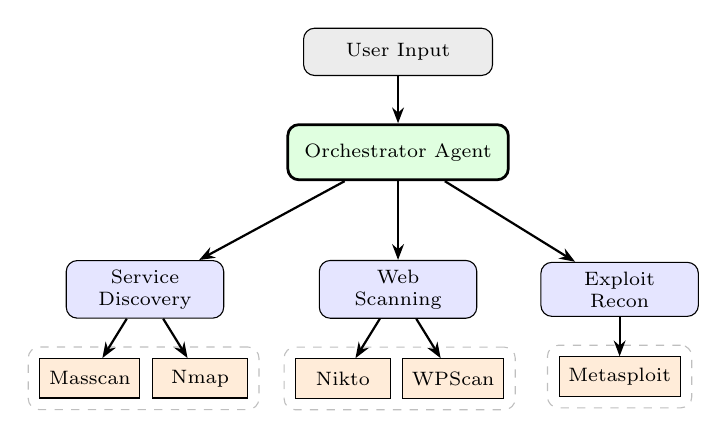
\begin{tikzpicture}[
    every node/.style={font=\scriptsize},
    orch/.style={rectangle, draw, rounded corners, minimum height=0.7cm, minimum width=2.8cm, align=center, fill=green!12, line width=1pt},
    agent/.style={rectangle, draw, rounded corners, minimum height=0.6cm, minimum width=2cm, align=center, fill=blue!10},
    tool/.style={rectangle, draw, minimum height=0.5cm, minimum width=1.2cm, align=center, fill=orange!15},
    user/.style={rectangle, draw, rounded corners, minimum height=0.6cm, minimum width=2.4cm, align=center, fill=gray!15},
    arr/.style={-{Stealth[length=2mm]}, thick},
    toolgroup/.style={rectangle, draw=gray!50, dashed, rounded corners, inner sep=4pt}
]
    \node (user) [user] {User Input};
    \node (orch) [orch, below=0.6cm of user] {Orchestrator Agent};

    \node (ws) [agent, below=1cm of orch] {Web\\Scanning};
    \node (sd) [agent, left=1.2cm of ws] {Service\\Discovery};
    \node (ex) [agent, right=0.8cm of ws] {Exploit\\Recon};

    \node (masscan) [tool, below=0.5cm of sd, xshift=-0.7cm] {Masscan};
    \node (nmap) [tool, below=0.5cm of sd, xshift=0.7cm] {Nmap};

    \node (nikto) [tool, below=0.5cm of ws, xshift=-0.7cm] {Nikto};
    \node (wpscan) [tool, below=0.5cm of ws, xshift=0.7cm] {WPScan};

    \node (msf) [tool, below=0.5cm of ex] {Metasploit};

    \node[toolgroup, fit=(masscan)(nmap)] {};
    \node[toolgroup, fit=(nikto)(wpscan)] {};
    \node[toolgroup, fit=(msf)] {};

    \draw[arr] (user) -- (orch);
    \draw[arr] (orch) -- (sd);
    \draw[arr] (orch) -- (ws);
    \draw[arr] (orch) -- (ex);
    \draw[arr] (sd) -- (masscan);
    \draw[arr] (sd) -- (nmap);
    \draw[arr] (ws) -- (nikto);
    \draw[arr] (ws) -- (wpscan);
    \draw[arr] (ex) -- (msf);
\end{tikzpicture}
\caption{V2 multi-agent architecture.}
\label{fig:architecture}
\end{figure}

The three sub-agents are:

\begin{itemize}[leftmargin=*]
    \item \textbf{Service Discovery Agent}: Owns Masscan (fast port discovery) and Nmap (in-depth service/OS fingerprinting). Instructed to run Masscan first for rapid reconnaissance, then Nmap for detailed analysis of discovered ports.
    \item \textbf{Web Scanning Agent}: Owns Nikto (general web server scanning) and WPScan (WordPress-specific vulnerability scanning). Selects tools based on detected web technologies.
    \item \textbf{Exploit Reconnaissance Agent}: Owns Metasploit tools for exploit search, CVE lookup, and exploit details. The agent supports two configurable modes: \emph{passive mode}, which searches for and reports matching exploits without executing them, and \emph{active mode}, which executes selected exploits against the target. To prevent accidental or malicious use against external systems, an internal guardrail restricts active mode to localhost targets. If the target address is not on the local network, the system refuses to enable active exploitation and falls back to passive reconnaissance. By default, the agent operates in passive mode.
\end{itemize}

% ============================================================
\section{Methodology}
\label{sec:methodology}
% ============================================================

The development followed an iterative design methodology. A monolithic architecture (V1) was first implemented and evaluated, its failure modes were identified, and a hierarchical multi-agent architecture (V2) was subsequently designed and evaluated in response to those findings.

The orchestrator agent uses OpenAI's GPT-4o as the underlying language model to handle task decomposition and re-planning, while the three sub-agents use GPT-4o mini for tool selection and command construction. Both models are accessed via the OpenAI API with the temperature parameter set to 0 to maximise determinism. This split balances reasoning capability at the orchestration layer, where planning decisions are more complex, with cost and latency efficiency at the sub-agent layer, where tasks are narrower in scope.

\subsection{V1: Single-Agent, Multi-Tool Architecture}

In the initial design, a single LLM agent was equipped with all security tools (Nmap, Nikto, WPScan, and Metasploit) as callable functions. The agent received the user query and was expected to select and invoke the appropriate tools in sequence.

\subsubsection{Identified Failure Modes}

Evaluation of V1 revealed three critical failure modes:

\begin{enumerate}[leftmargin=*]
    \item \textbf{No separation of concerns}: The agent was responsible for understanding the query, selecting among disparate tools, constructing syntactically correct commands for each tool, parsing heterogeneous outputs, and deciding next steps. Handling all this within a single reasoning chain overloaded the agent's planning capacity.

    \item \textbf{Context exhaustion}: Security tool outputs (especially Nmap and WPScan) can be verbose, often spanning thousands of tokens. After one or two tool executions, the agent's effective context window was consumed by raw output, leaving insufficient capacity for reasoning about subsequent steps.

    \item \textbf{Redundant tool invocation}: Because all tools were attached directly to a single agent, and previously returned outputs remained in its context, the agent frequently re-invoked the same tool with substantively identical arguments rather than progressing to the next stage of the workflow. In several runs the agent looped on Nmap or Nikto for multiple iterations before either exhausting its context or producing a partial report. This pattern is consistent with documented failure modes of LLM tool use under context overload.

    \item \textbf{Constrained tool surface, but no scope isolation}: Tools were exposed to the agent as Python functions with explicit, typed parameters rather than via direct shell access. This prevented arbitrary command injection by the agent, but it did not prevent the agent from overusing the tools it did have access to (e.g., repeatedly invoking the same scanner). V1 therefore had safe \emph{tool execution} but inefficient \emph{tool selection}.
    
\end{enumerate}

These failure modes motivated the multi-agent redesign.

\subsection{V2: Multi-Agent Orchestration}

The V2 architecture addresses each V1 failure mode through hierarchical decomposition:

\subsubsection{Orchestrator Agent}

The orchestrator serves as the entry point and coordinator. Its responsibilities are:

\begin{enumerate}[leftmargin=*]
    \item \textbf{Intent classification}: Distinguish informational queries (e.g., ``What is a SYN scan?'') from execution requests (e.g., ``Scan 192.168.1.0/24 for open ports'') using keyword heuristics and LLM fallback.
    \item \textbf{Task decomposition}: Break execution requests into an ordered task list (e.g., \texttt{[service\_discovery, web\_scan, exploit\_recon]}).
    \item \textbf{Sub-agent delegation}: Route each task to the appropriate sub-agent, passing relevant context (target, prior findings).
    \item \textbf{Dynamic re-planning}: After each sub-agent completes, the orchestrator evaluates results and updates the task plan. For example, if service discovery reveals a web server on port 80, the orchestrator adds web scanning to the plan.
    \item \textbf{Result synthesis}: Aggregate structured results from all sub-agents into a coherent final report.
\end{enumerate}

The orchestrator does \emph{not} have direct access to any security tools. It can only communicate with sub-agents, enforcing strict separation of concerns.

\subsubsection{Sub-Agent Design}

Each sub-agent is an agent with:

\begin{itemize}[leftmargin=*]
    \item A focused system prompt describing its domain and tools.
    \item Tool bindings for only its own tools (e.g., the Service Discovery agent cannot invoke WPScan).
    \item An LLM-based output parser that converts raw tool output into a Pydantic-validated structured result.
\end{itemize}

\subsubsection{Configurable Human-in-the-Loop Interrupts}

The V2 architecture supports configurable \emph{tool-call interrupts}. Users can specify which tool invocations require explicit human approval before execution. For example, a user may allow Masscan scans to proceed automatically but require confirmation before Nmap aggressive scans or Metasploit queries. This is implemented as an interrupt layer between the sub-agent's tool selection and tool execution.

\subsubsection{Parallel Tool Execution}

Within a sub-agent, independent tool calls can be executed in parallel. For instance, the Web Scanning agent can run Nikto and WPScan concurrently against the same target when both are deemed necessary. This reduces end-to-end scan time without sacrificing result quality.

\subsection{Workflow Enforcement}

Rather than enforcing a rigid linear sequence, the orchestrator imposes \emph{prerequisite constraints} on sub-agent invocation. Specifically, the Web Scanning agent can only be invoked after the Service Discovery agent has been called at least once, and the Exploit Reconnaissance agent can only be invoked after at least one scanning agent (Web Scanning or Service Discovery) has produced vulnerability findings. Beyond these prerequisites, the orchestrator retains full flexibility in its execution plan. For instance, it may invoke Service Discovery, then Web Scanning, and then return to Service Discovery for deeper analysis of newly relevant ports before proceeding to Exploit Reconnaissance. This design balances safety
with the dynamic, iterative nature of real-world security assessments.

\subsection{Implementation Details}
\label{sec:implementation}

The V2 system is implemented in Python. Agent orchestration is built on LangChain's DeepAgents. Tools are exposed as custom Python functions with explicit typed parameters; no agent has shell access. Structured outputs from each sub-agent are validated against Pydantic schemas before being returned to the orchestrator. Underlying scanners are invoked via their standard CLIs (Masscan, Nmap, Nikto, WPScan) or framework APIs (Metasploit RPC).


% ============================================================
\section{Evaluation}
\label{sec:evaluation}
% ============================================================

The architectures were evaluated on a controlled vulnerable target to compare V1 and V2 along three dimensions: end-to-end execution time, tool invocation behaviour, and the completeness of the final report. The target was a Damn Vulnerable WordPress (DVWP) deployment~\cite{dvwp}, a Docker-based vulnerable WordPress instance that exposes a representative mix of misconfigurations, outdated components, and exploitable endpoints. All scans were issued with the same natural-language prompt: a request to perform reconnaissance, web vulnerability scanning, and exploit lookup against \texttt{localhost:31337}.

\subsection{Experimental Setup}

Both V1 and V2 were configured to use the same underlying tool implementations (Masscan, Nmap, Nikto, WPScan, and Metasploit) and were run against an identical DVWP instance on the same host. V1 used a single GPT-4o agent with all tools attached directly; V2 used the orchestrator/sub-agent split described in Section~\ref{sec:methodology}, with GPT-4o as the orchestrator and GPT-4o mini in each sub-agent. Temperature was fixed at zero for all agents. Each configuration was executed multiple times to account for non-determinism in tool selection, and per-run logs of tool invocations and final reports were retained for inspection.

\subsection{Metrics}

The following metrics were collected:

\begin{itemize}[leftmargin=*]
    \item \textbf{End-to-end execution time}: wall-clock time from user prompt to final report.
    \item \textbf{Total tool calls issued}: the number of tool invocations made by the agent(s) per run.
    \item \textbf{Redundant tool calls}: invocations of the same tool with substantively similar arguments within a single run.
    \item \textbf{Tool invocation accuracy}: the fraction of tool calls that were both syntactically valid and appropriate for the current sub-task, judged against a reference workflow.
    \item \textbf{Final report completeness}: whether the report included findings from each expected stage (service discovery, web scanning, and exploit reconnaissance).
\end{itemize}

\subsection{Results}

Table~\ref{tab:v1_vs_v2} summarises the comparison between the two architectures on the DVWP target.

\begin{table}[htbp]
\centering
\caption{V1 vs.\ V2 on the DVWP target.}
\label{tab:v1_vs_v2}
\small
\begin{tabular}{lcc}
\toprule
\textbf{Metric} & \textbf{V1 (single-agent)} & \textbf{V2 (multi-agent)} \\
\midrule
End-to-end time (s)         & TODO  & TODO \\
Tool calls per run          & TODO  & TODO \\
Redundant tool calls        & TODO  & TODO \\
Tool invocation accuracy    & TODO\% & TODO\% \\
Reports covering all stages & TODO  & TODO \\
\bottomrule
\end{tabular}
\end{table}

% ============================================================
\section{Observations and Discussion}
\label{sec:discussion}
% ============================================================

\subsection{Prompt Engineering for Reliable Tool Invocation}

In V1, the single agent frequently bypassed tools and fabricated plausible-looking scan outputs, even when explicitly instructed to use the provided tools. This hallucination behaviour worsened as more tool definitions were added to its context.

The transition to V2 alleviated much of this through the separation of concerns, but sub-agent prompts still required iterative optimisation. Reliable tool invocation was achieved through three strategies: (1) a \emph{forced-execution directive} prohibiting output generation without at least one tool call, (2) front-loading tool descriptions and usage examples in the system prompt, and (3) including negative examples of hallucinated responses for the agent to avoid. These prompt-level interventions, combined with each sub-agent's reduced cognitive load, were essential to eliminating fabricated outputs.

\subsection{Benefits of Multi-Agent Separation}

The core finding is that decomposing a multi-tool security workflow across specialised agents yields substantial improvements in reliability and completeness. The orchestrator-sub-agent hierarchy mirrors how human security teams operate: a lead analyst coordinates specialists, each of whom focuses on a specific assessment domain.

The separation of concerns provides three specific benefits. First, each sub-agent's context contains only its own tool definitions and outputs, avoiding the context exhaustion observed in V1. Second, sub-agents reason only within their domain, reducing the probability of tool-call hallucination. Third, new tools can be added to a sub-agent, or new sub-agents introduced, without modifying the orchestrator's core logic.

\subsection{Parallel Execution Benefits}

Parallel tool execution within the Web Scanning agent reduced scan time by a meaningful margin when both Nikto and WPScan were invoked, compared to sequential execution.

% ============================================================
\section{Conclusion and Future  Work}
\label{sec:conclusion}
% ============================================================

A multi-agent cybersecurity scanning system is presented that evolves from a monolithic single-agent design to a hierarchical orchestrator and sub-agent architecture. Implemented using LangChain’s agent framework, the approach shows that separating concerns across specialised agents reduces tool-call hallucination, mitigates context exhaustion, and improves scan completeness. Observations from the development process highlight the importance of prompt optimisation for reliable tool invocation, structured output schemas for inter-agent context passing, and configurable human-in-the-loop interrupts for building user confidence, which emerged as a decisive factor in willingness to adopt the system. A configurable passive and active Metasploit mode, constrained by a localhost-only guardrail for active exploitation, provides a practical safety boundary for responsible use.

Future work includes: (1) expanding the tool set to include additional scanners (for example, SQLMap and headless Burp Suite); (2) conducting a formal user study to quantify the impact of human-in-the-loop controls on trust and adoption; and (3) extending the system with a background monitoring agent that continuously performs scheduled scans and re-assessments to detect newly introduced or emerging vulnerabilities, while surfacing only actionable changes to the user.

\bibliographystyle{ACM-Reference-Format}
\begin{thebibliography}{99}

\bibitem{nmap}
G.~F.~Lyon, ``Nmap Network Scanning: The Official Nmap Project Guide,''
Insecure.Com LLC, 2009. [Online]. Available: \url{https://nmap.org/book/}

\bibitem{deng2023pentestgpt}
G.~Deng \emph{et al.}, ``PentestGPT: An LLM-empowered automatic penetration testing tool,''
\emph{arXiv preprint arXiv:2308.06782}, 2023. [Online]. Available: \url{https://arxiv.org/abs/2308.06782}

\bibitem{fang2024llmagents}
R.~Fang \emph{et al.}, ``LLM agents can autonomously hack websites,''
\emph{arXiv preprint arXiv:2402.06664}, 2024. [Online]. Available: \url{https://arxiv.org/abs/2402.06664}

\bibitem{xu2024autoattacker}
J.~Xu, J.~W.~Stokes, G.~McDonald, X.~Bai, D.~Marshall, S.~Wang, A.~Swaminathan, and Z.~Li,
``AutoAttacker: A Large Language Model Guided System to Implement Automatic Cyber-attacks,''
\emph{arXiv preprint arXiv:2403.01038}, 2024. [Online]. Available: \url{https://arxiv.org/abs/2403.01038}

\bibitem{shen2024pentestagent}
X.~Shen, L.~Wang, Z.~Li, Y.~Chen, W.~Zhao, D.~Sun, J.~Wang, and W.~Ruan,
``PentestAgent: Incorporating LLM Agents to Automated Penetration Testing,''
\emph{arXiv preprint arXiv:2411.05185}, 2024. [Online]. Available: \url{https://arxiv.org/abs/2411.05185}

\bibitem{kong2025vulnbot}
H.~Kong, D.~Hu, J.~Ge, L.~Li, T.~Li, and B.~Wu,
``VulnBot: Autonomous Penetration Testing for A Multi-Agent Collaborative Framework,''
\emph{arXiv preprint arXiv:2501.13411}, 2025. [Online]. Available: \url{https://arxiv.org/abs/2501.13411}

\bibitem{henke2025autopentest}
J.~Henke,
``AutoPentest: Enhancing Vulnerability Management With Autonomous LLM Agents,''
\emph{arXiv preprint arXiv:2505.10321}, 2025. [Online]. Available: \url{https://arxiv.org/abs/2505.10321}

\bibitem{ginige2025autopentester}
Y.~Ginige, A.~Niroshan, S.~Jain, and S.~Seneviratne, ``AutoPentester: An LLM Agent-based Framework for Automated Pentesting,''
\emph{arXiv preprint arXiv:2510.05605}, 2025. [Online]. Available: \url{https://arxiv.org/abs/2510.05605}

\bibitem{hong2023metagpt}
S.~Hong \emph{et al.}, ``MetaGPT: Meta programming for a multi-agent collaborative framework,''
\emph{arXiv preprint arXiv:2308.00352}, 2023. [Online]. Available: \url{https://arxiv.org/abs/2308.00352}

\bibitem{boiko2023emergent}
D.~A.~Boiko, R.~MacKnight, and G.~Gomes, ``Emergent autonomous scientific research capabilities of large language models,''
\emph{arXiv preprint arXiv:2304.05332}, 2023. [Online]. Available: \url{https://arxiv.org/abs/2304.05332}

\bibitem{wu2023autogen}
Q.~Wu \emph{et al.}, ``AutoGen: Enabling next-gen LLM applications via multi-agent conversation,''
\emph{arXiv preprint arXiv:2308.08155}, 2023. [Online]. Available: \url{https://arxiv.org/abs/2308.08155}

\bibitem{yin2025agentframeworks}
Z.~Yin, C.~Gao, C.~Fan, W.~Yang, Y.~Xue, and L.~Zhang, ``A Comprehensive Empirical Evaluation of Agent Frameworks on Code-centric Software Engineering Tasks,''
\emph{arXiv preprint arXiv:2511.00872}, 2025. [Online]. Available: \url{https://arxiv.org/abs/2511.00872}

\bibitem{langgraph_workflows_agents}
LangChain, ``Workflows and agents (LangGraph documentation),'' 2025.
[Online]. Available: \url{https://docs.langchain.com/oss/python/langgraph/workflows-agents}

\bibitem{crewai2024}
CrewAI, ``CrewAI: Framework for orchestrating role-playing autonomous AI agents,'' 2024.
[Online]. Available: \url{https://github.com/crewAIInc/crewAI}

\bibitem{dvwp}
V.~Kamil, ``DVWP: Damn Vulnerable WordPress Project,'' GitHub repository, 2024.
[Online]. Available: \url{https://github.com/vavkamil/dvwp}

% \bibitem{yao2023react}
% S.~Yao \emph{et al.}, ``ReAct: Synergizing reasoning and acting in language models,''
% in \emph{Proc.\ ICLR}, 2023. [Online]. Available: \url{https://openreview.net/forum?id=WE_vluYUL-X}

\end{thebibliography}

\end{document}
